\begin{figure}
    \begin{center}
    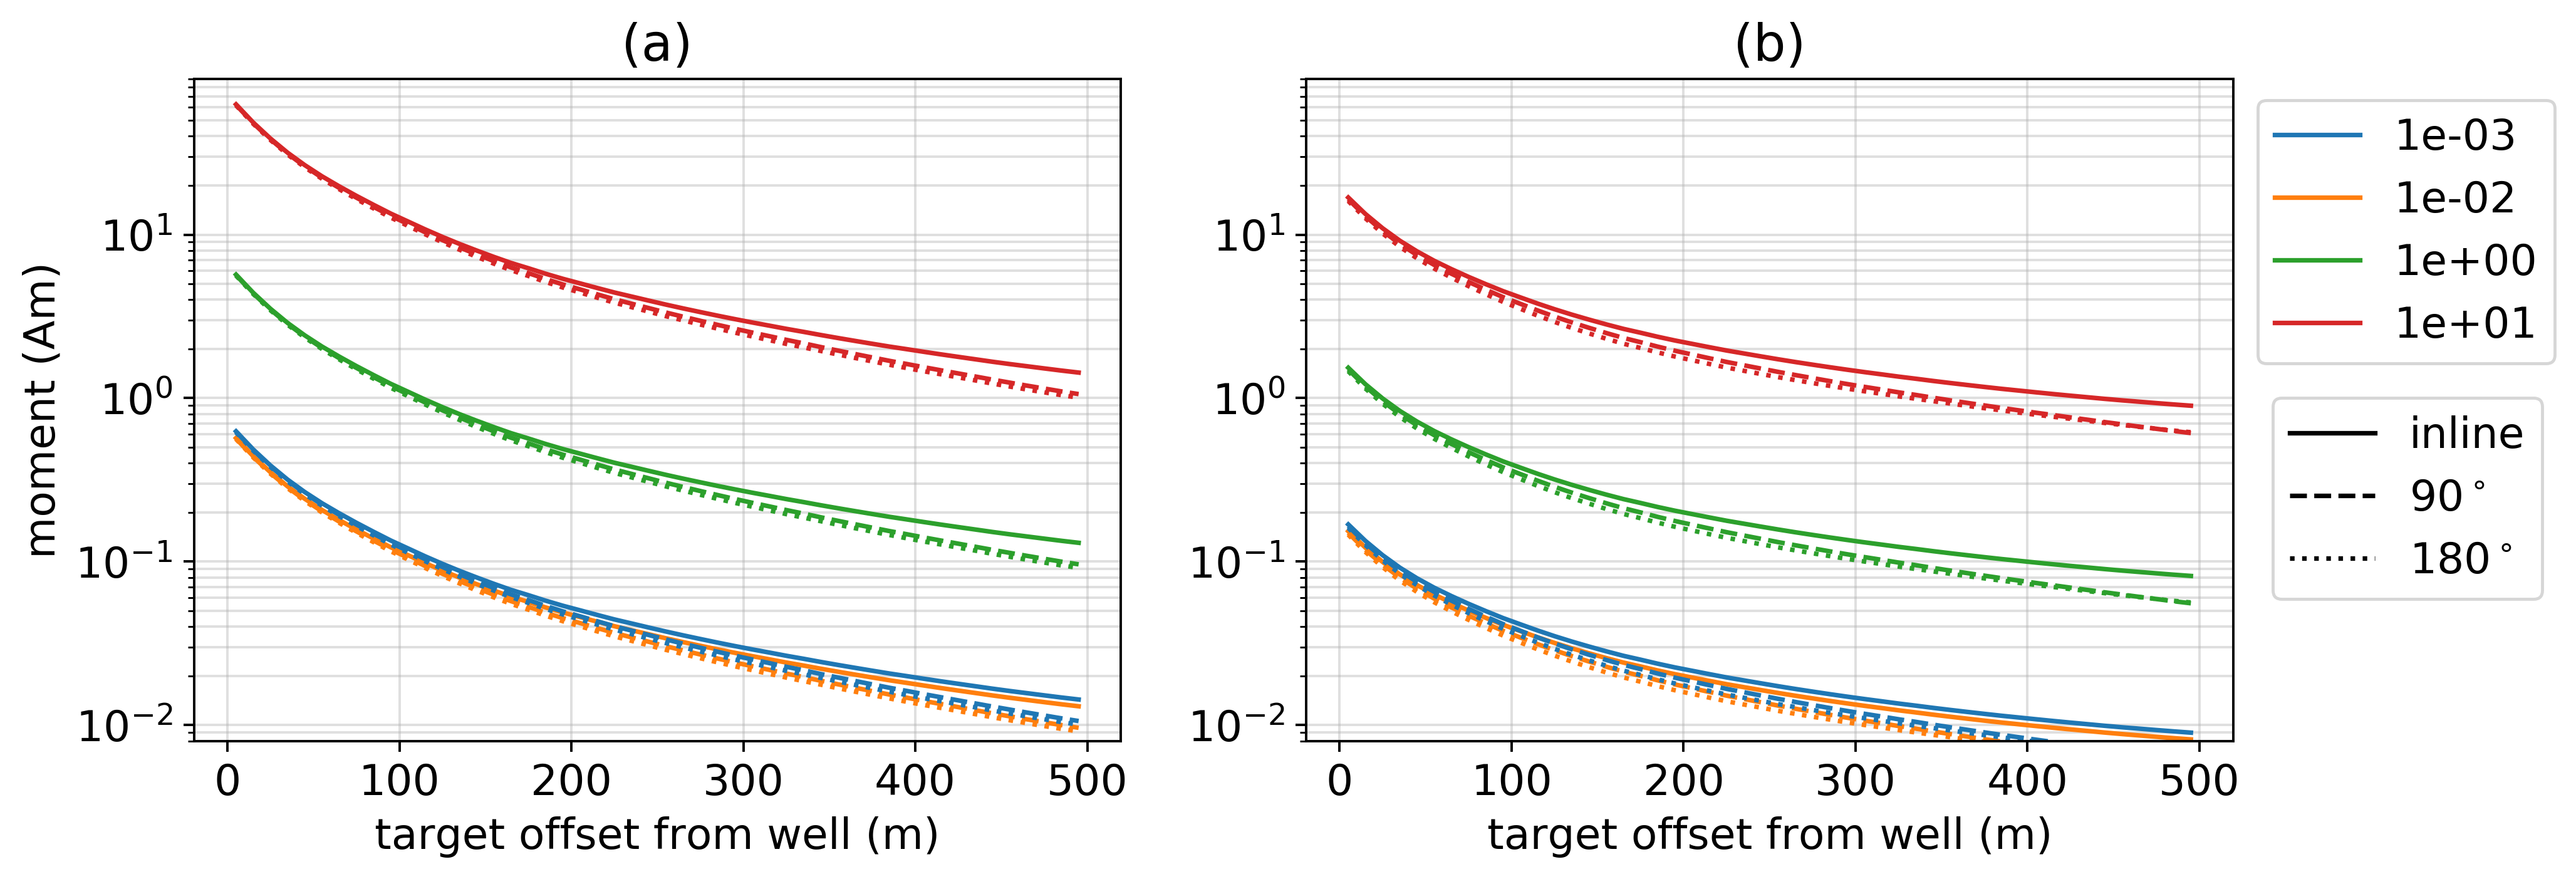
\includegraphics[width=\textwidth]{figures/dc_casing/excitation_3D.png}
    \end{center}
\caption{
    Integrated anomalous current density (excitation), as defined in equation \ref{eq:excitation},
    for a 50m $\times$ 50m $\times$ 25m target at 900m depth in a DC experiment with the positive electrode
    (a) downhole at 912.5m depth, and (b) a top-casing electrode. The return electrode is positiond on the
    surface 500m from the well. Each line color indicates a different target-conductivity. The different line
    styles correspond to different target azimuths relative to the plane of the source electrodes and correspond
    to those show in Figure \ref{fig:primary_3D}. The solid line indicates a target inline with the source,
    the dashed is $90^\circ$ from the source, and the dotted line is $180^{\circ}$ from the source. Offset is
    calculated from the center of the well to the edge of the target closest to the well.
}
\label{fig:excitation_3D}
\end{figure}
